\section{What was your first big trip?}
The trip I will describe here is one I took the summer of 1970.
I had graduated from high school in June.
On July 6 a group of thirteen students and one teacher from LMS arrived by plane in Rome, Italy.
We were part of a larger group of students touring and studying with the Foreign Study League.
My memory is that the total group numbered close to 200 students and teachers.
Our time in Europe was divided between Italy, Switzerland, France, and England.
Each country had its set of classes and curriculum.
I earned my first college credits with these classes.
Attached is a photo of me at the airport ready to fly.
My face is sunburned from spending some time at the shore without enough sun screen.
One other girl in our group and I wore our hair up with a covering.
The other girls wore their hair down with or without a covering.
\begin{figure}
\centering
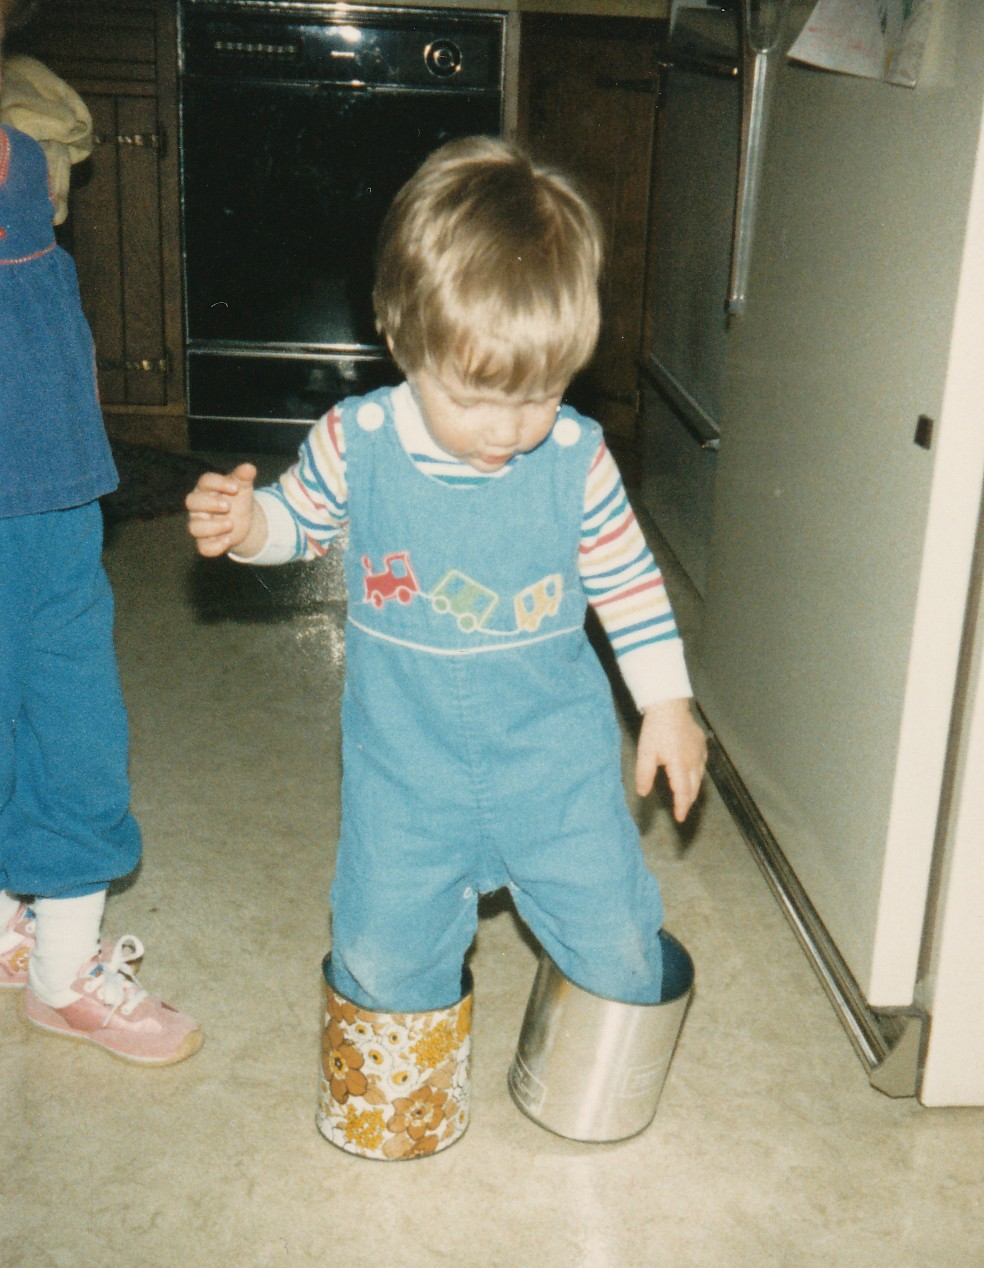
\includegraphics[width=0.9\textwidth]{childhood/16.jpg}
\caption{
Ready to fly to Italy
}
\end{figure}

Our first lodging in Rome was at a Catholic Convent.
Part of the day was spent in class and the rest the day we went on guided tours of museums, churches, ruins such as Acropolis, Parthenon, Pompeii, and the Vatican.
We attended an evening performance of Aida.
We watched this performance outdoors on a set in the Roman ruins.
Watching a segment of the opera just now I remember the sense of awe and amazement I felt watching such a spectacular performance which included live animals.
It was likely one of the first live opera performances I had seen.
\begin{figure}
\centering
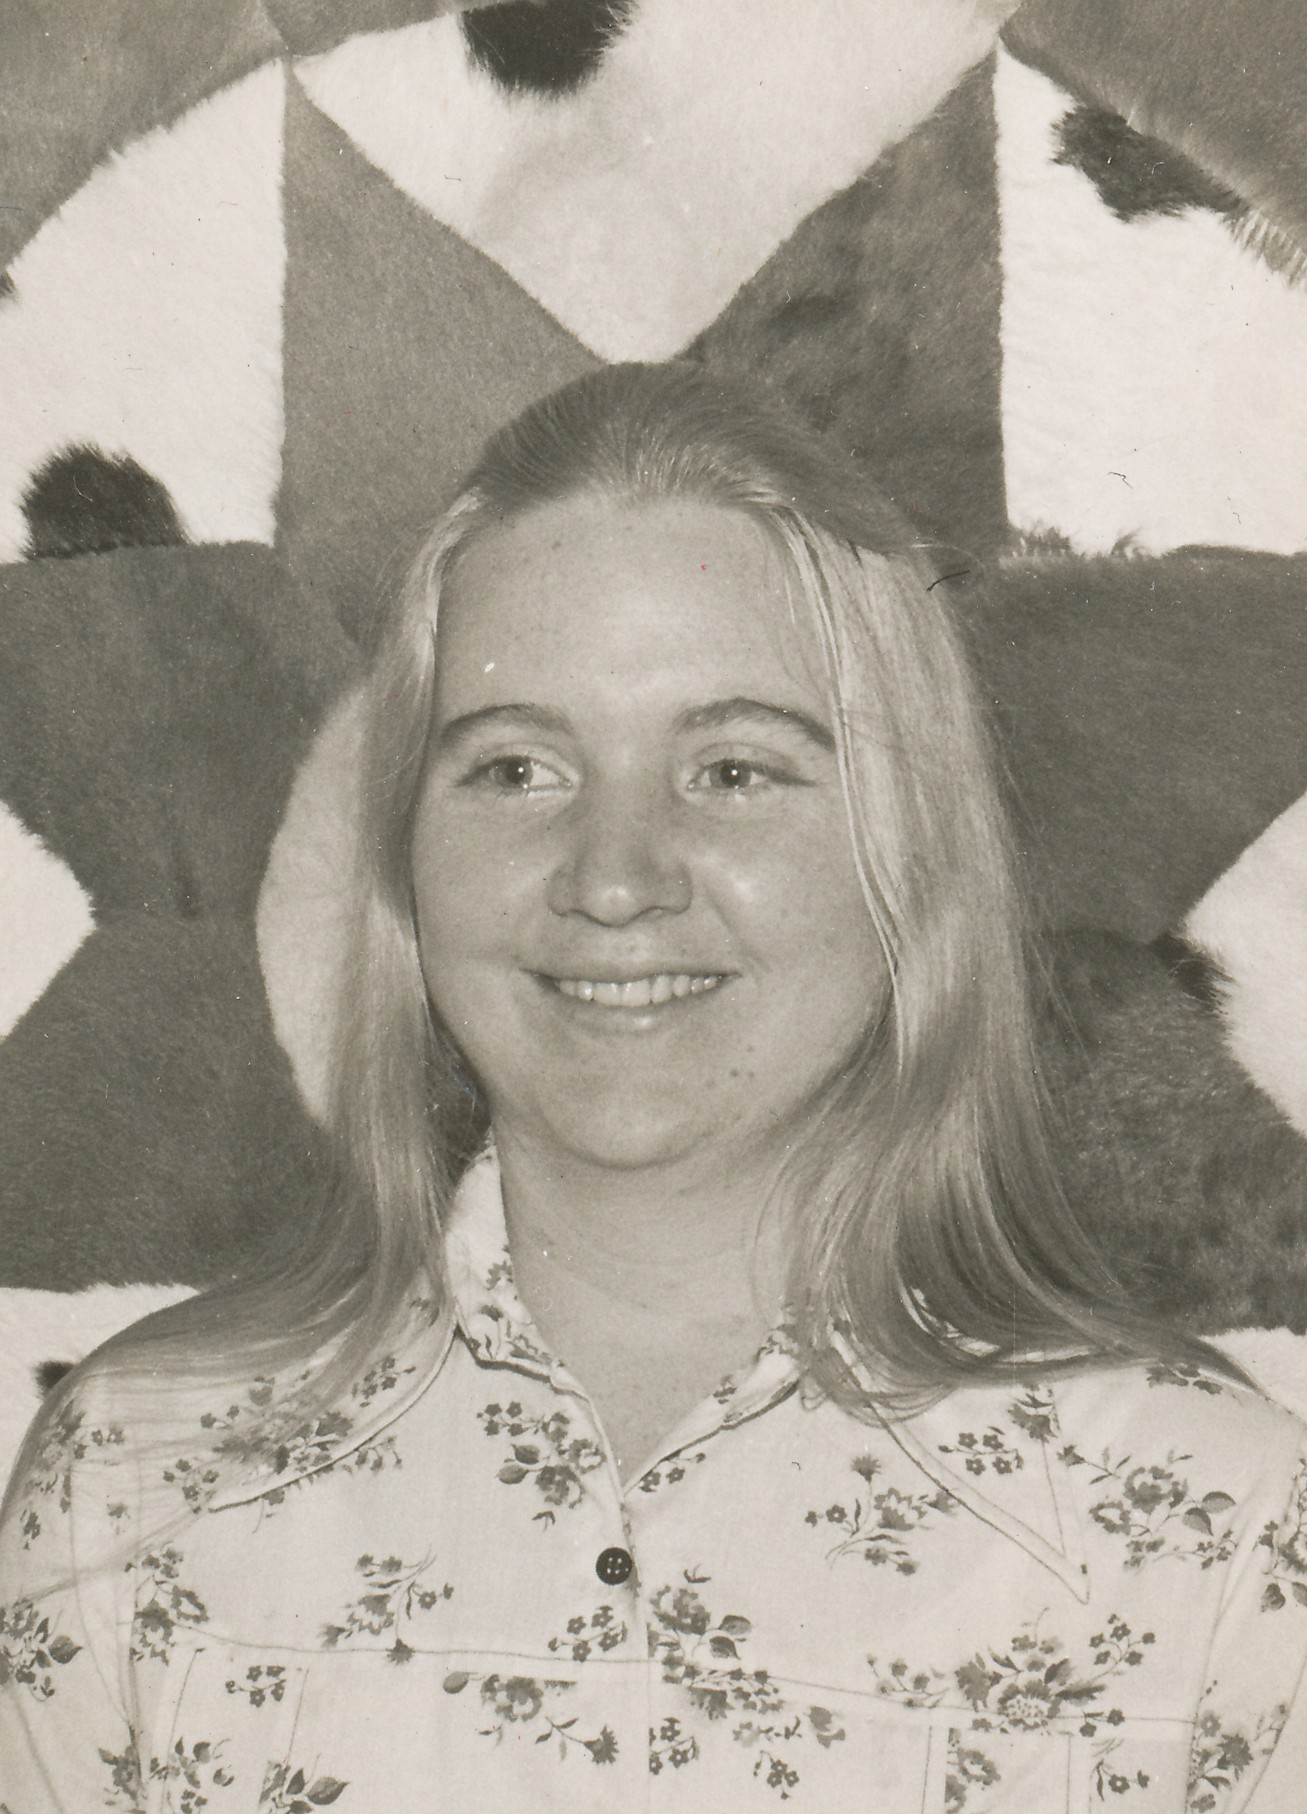
\includegraphics[width=0.9\textwidth]{childhood/17.jpg}
\caption{
Schedule for four countries.
}
\end{figure}
Next we traveled by bus through Florence and up through the mountains, through the Saint Bernard pass into Switzerland.
It was snowing in the higher elevations as the buses climbed the switchback roads up and over the pass.
The Swiss mountains were majestic and snowcapped in comparison to the worn down Appalachian Mountains I knew in Pennsylvania.
Our base lodging was a school in the city of Lucerne.
Since the dorms available were filled, our LMS group and a small group from Kentucky were given lodging in a chalet like building up in the mountains.
It was surrounded with meadows, home to the brown Swiss cows.
I remember walking through the beautifully illustrated Chapel Bridge.
(It was later burned but has been replaced.
) We traveled to Berne and Zurich.
Saw statues of Zwingli and William Tell.
I purchased a cuckoo clock and had it sent home to my parents.
When I left home my mother gave it back to me.
A favorite memory from my time in Switzerland was an evening walk in the mountain meadows and hearing the cow bells before we gathered for a fondue dinner.

France was next.
The world here seemed larger than the one we left in Switzerland.
We had lodging in Versailles and visited the palace there.
We visited the Notre Dame Cathedral, the Eiffel Tower, and the Louvre art museum.
We had a boat ride on the Seine River at night.
I remember walking through Montmartre and enjoying the ever present sticks of French bread.

\begin{figure}
\centering
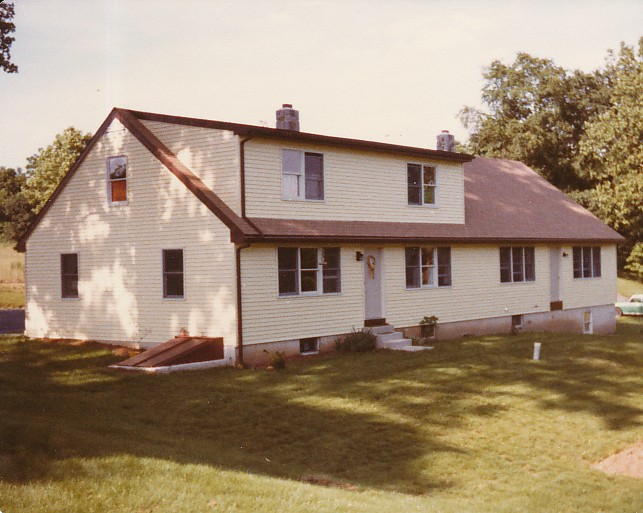
\includegraphics[width=0.9\textwidth]{childhood/18.jpg}
\caption{
Small group in London
}
\end{figure}
Then we were off to the final country on the agenda, England.
We traveled across the English Channel in a Hovercraft.
I learned that these vehicles transported cars and people across the channel from 1968 to 2000.
Our lodging was in Reading.

But we spent lots of time in London where we saw and heard Big Ben.
Again there were visits to many cathedrals, museums, and palaces.
I watched a Shakespeare play and fell in love with Johann Strauss's Blue Danube Waltz.

On one of the Sundays we were in London, Dan Wenger herded the LMS group to visit the London Mennonite Center.
Unfortunately the Kreider family was state side and we ended up eating our lunch in a nearby park.
Then we were once more in the blue skies heading home leaving the world of kings and queens, artists, and the Alps behind.
Four weeklong classes completed for an A, which was a good start for my four years of college grades.
\begin{figure}
\centering
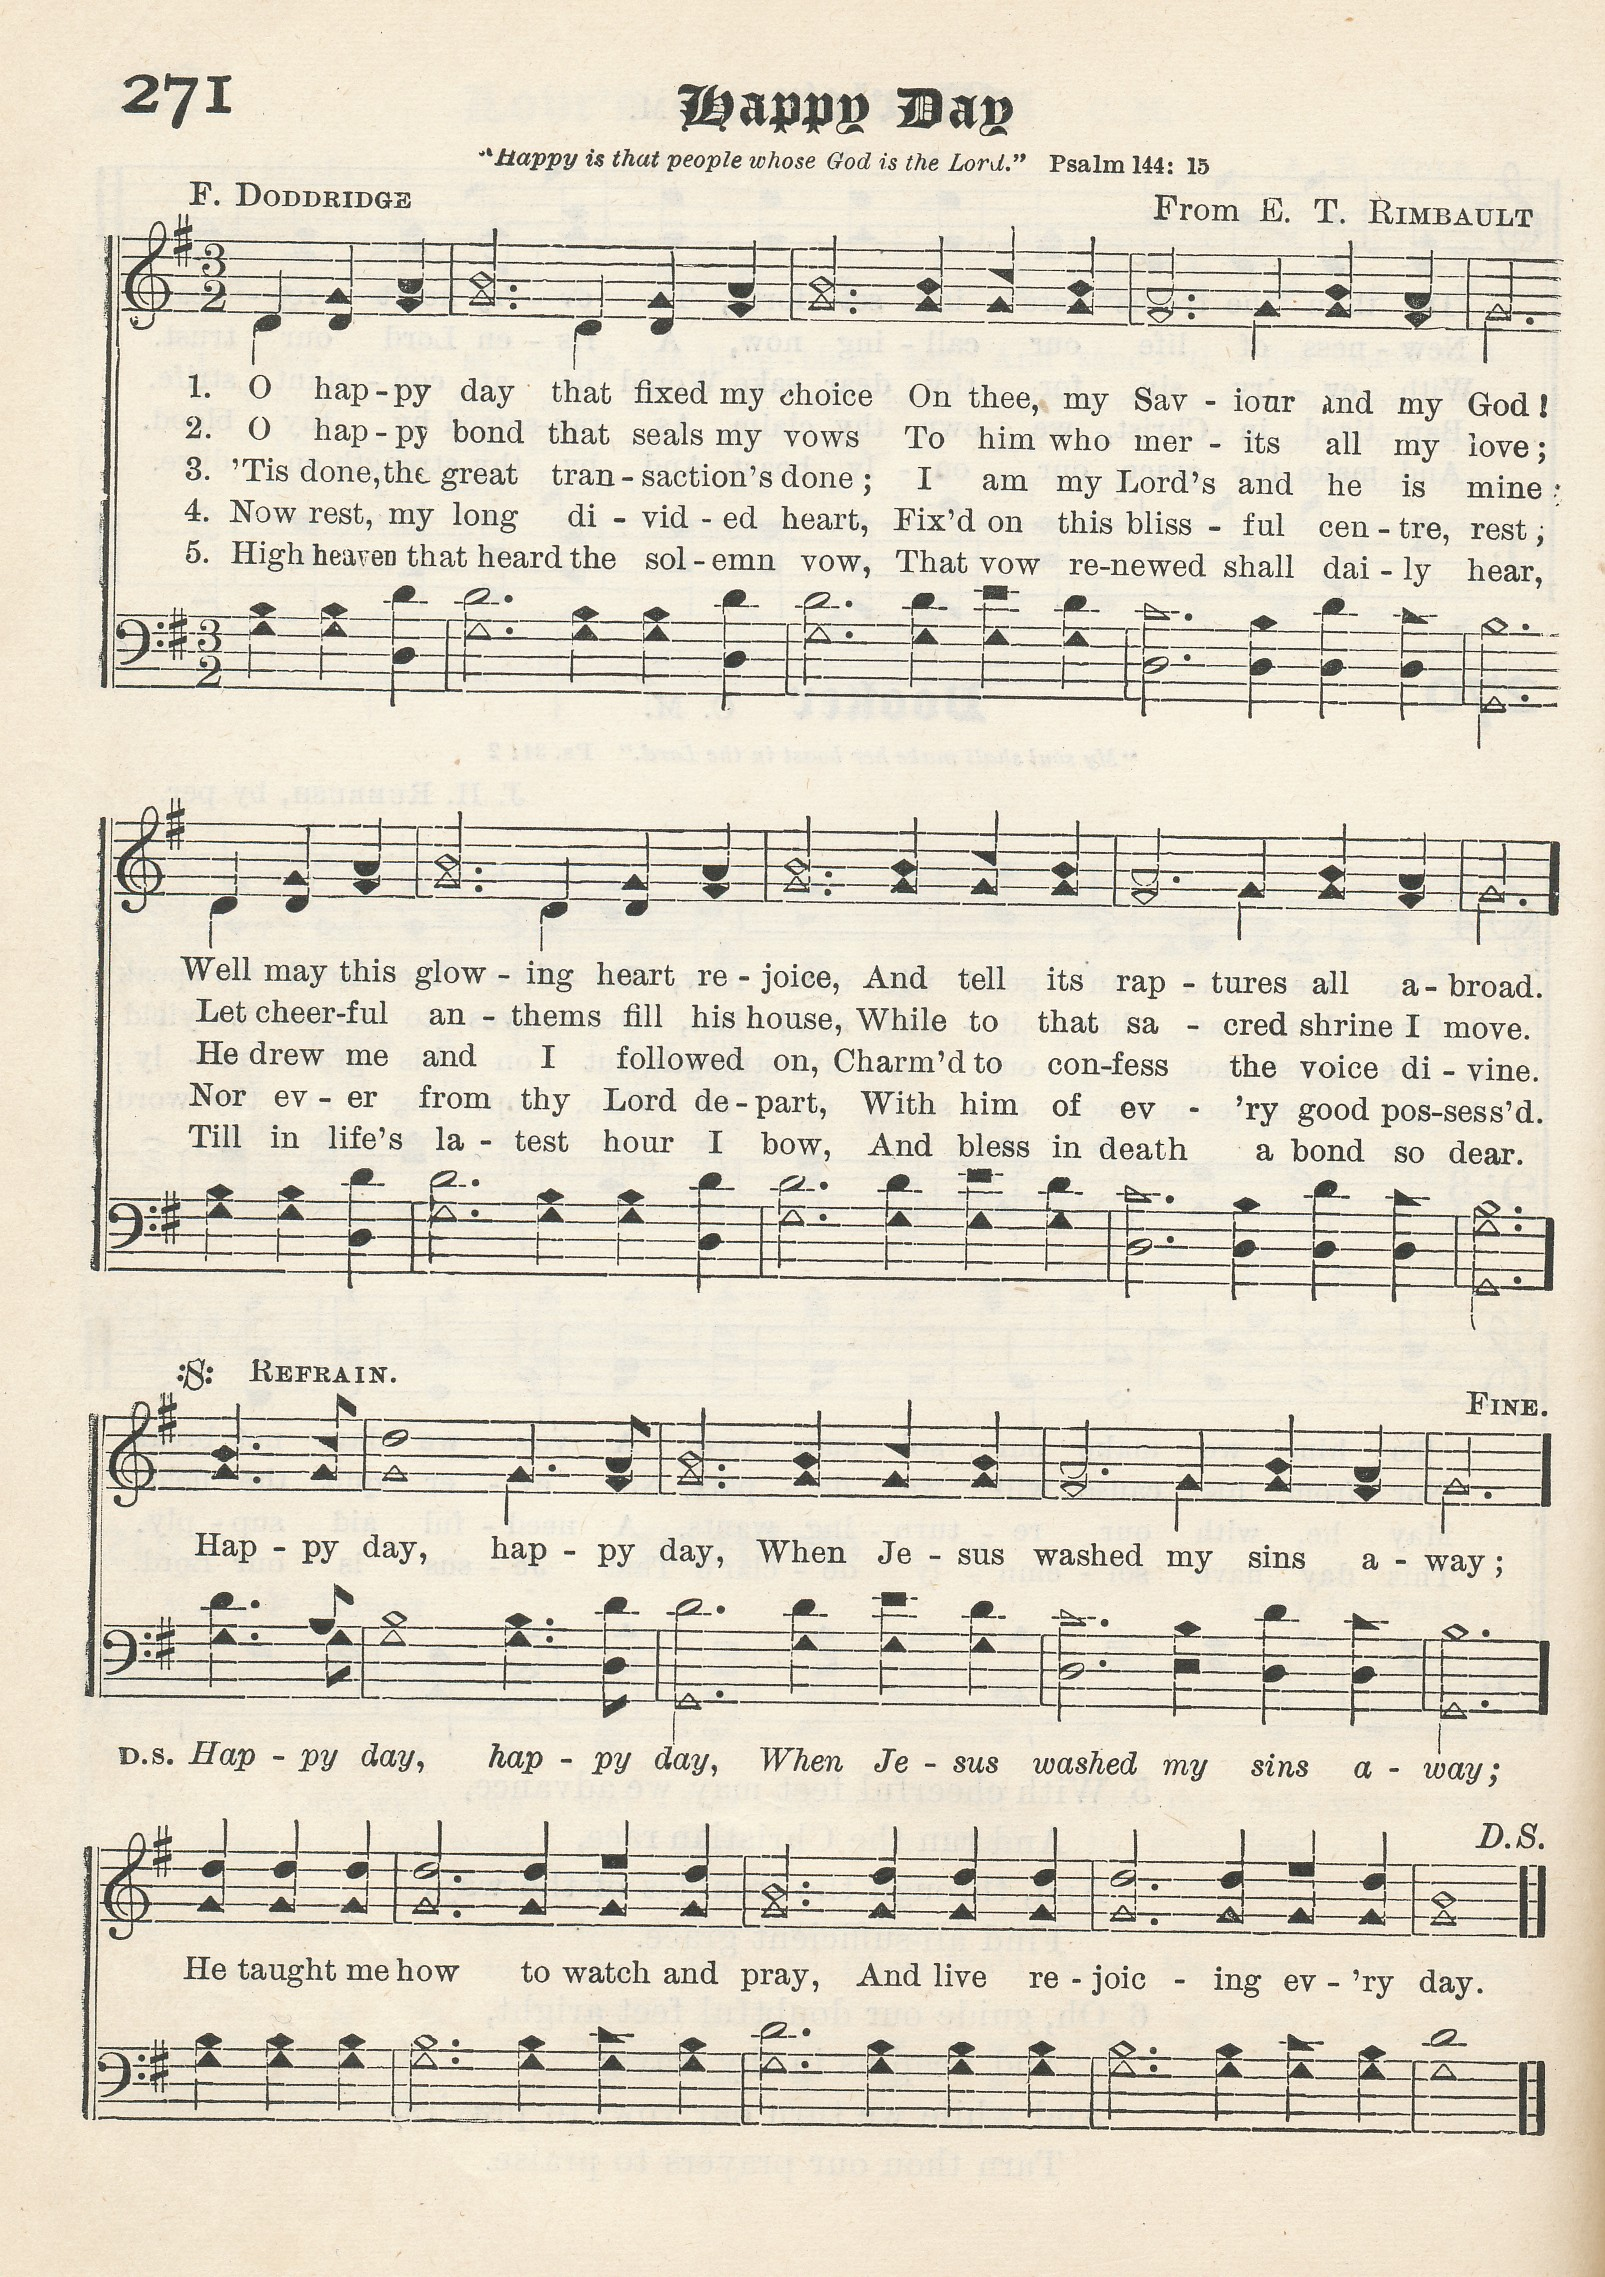
\includegraphics[width=0.9\textwidth]{childhood/19.jpg}
\caption{
Large group taken in Reading England.
}
\end{figure}
I'm grateful that my parents gave permission for me to participate in this experience.

\textbf{From Abby -} What an amazing trip Mom! Two small things of note, Aida was also one of the first "live" operas I ever saw, but I viewed it in a movie theater in Chicago as it was performed live at the Metropolitan Opera in New York.
And I also remember walking across the Chapel bridge in Lucerne, although probably the reconstructed version, since that would have been during my high school trip to Germany and Switzerland in 2000.
